\documentclass[a4paper,12pt,oneside]{book}

%-------------------------------Start of the Preable------------------------------------------------
\usepackage[english]{babel}
\usepackage{blindtext}
%packagr for hyperlinks
\usepackage{hyperref}
\hypersetup{
    colorlinks=true,
    linkcolor=blue,
    filecolor=magenta,      
    urlcolor=cyan,
}

\urlstyle{same}
%use of package fancy header
\usepackage{fancyhdr}
\setlength\headheight{26pt}
\fancyhf{}
%\rhead{
\includegraphics[width=1cm]{logo}}
\lhead{\rightmark}
\rhead{
\includegraphics[width=1cm]{logo}}
\fancyfoot[RE, RO]{\thepage}
\fancyfoot[CE, CO]{\href{http://www.e-yantra.org}{www.e-yantra.org}}

\pagestyle{fancy}

%use of package for section title formatting
\usepackage{titlesec}
\titleformat{\chapter}
  {\Large\bfseries} % format
  {}                % label
  {0pt}             % sep
  {\huge}           % before-code
 
%use of package tcolorbox for colorful textbox
\usepackage[most]{tcolorbox}
\tcbset{colback=cyan!5!white,colframe=cyan!75!black,halign title = flush center}

\newtcolorbox{mybox}[1]{colback=cyan!5!white,
colframe=cyan!75!black,fonttitle=\bfseries,
title=\textbf{\Large{#1}}}

%use of package marginnote for notes in margin
\usepackage{marginnote}

%use of packgage watermark for pages
%\usepackage{draftwatermark}
%\SetWatermarkText{
\includegraphics{logo}}
\usepackage[scale=2,opacity=0.1,angle=0]{background}
\backgroundsetup{
contents={
\includegraphics{logo}}
}

%use of newcommand for keywords color
\usepackage{xcolor}
\newcommand{\keyword}[1]{\textcolor{red}{\textbf{#1}}}

%package for inserting pictures
\usepackage{graphicx}
\graphicspath{ {images/} }

%package for highlighting
\usepackage{color,soul}


\usepackage{tikz}

\newcommand{\ExternalLink}{%
    \tikz[x=1.2ex, y=1.2ex, baseline=-0.05ex]{% 
        \begin{scope}[x=1ex, y=1ex]
            \clip (-0.1,-0.1) 
                --++ (-0, 1.2) 
                --++ (0.6, 0) 
                --++ (0, -0.6) 
                --++ (0.6, 0) 
                --++ (0, -1);
            \path[draw, 
                line width = 0.5, 
                rounded corners=0.5] 
                (0,0) rectangle (1,1);
        \end{scope}
        \path[draw, line width = 0.5] (0.5, 0.5) 
            -- (1, 1);
        \path[draw, line width = 0.5] (0.6, 1) 
            -- (1, 1) -- (1, 0.6);
        }
    }


%new command for table
\newcommand{\head}[1]{\textnormal{\textbf{#1}}}


%----------------------End of the Preamble---------------------------------------


\begin{document}

%---------------------Title Page------------------------------------------------
\begin{titlepage}
\raggedright
{\Large eYSIP 2017\\[1cm]}
{\Huge\scshape Modular Robot \\[.1in]}
\vfill
\begin{flushright}
{\large Srijal Poojari \\}
{\large Madhav Wagh \\}
{\large Mentors: Pushkar Raj, Aditya Panwar and Fayyaz Pocker \\}
{\large Duration of Internship: $ 22/05/2017-07/07/2017 $ \\}
\end{flushright}

{\itshape 2017, e-Yantra Publication}
\end{titlepage}
%-------------------------------------------------------------------------------

\chapter[Project Tag]{Modular Robot}
\section*{Abstract}
  This project is about homogeneous modular robotic modules, 
  which are coupled using mechanical and magnetic coupling. 
  The goal of the project is to explore existing modular robots, mainly the Dtto: Modular robot and expanding its capabilities. \\
  The modules are initially tested in a simulation environment for their feasibility (V-REP) and sensors (ToF) are interfaced to the modules for smart sensing and decision making. Snake motion, wheel motion, coupling/decoupling, obstacle detection and avoidance are achieved in practice. 

\subsection*{Completion status}
\textbf{Tasks given: }
\begin{enumerate}
\item Getting familiar with existing Models of Modular Robots\\ Status: Completed
\\ Details: Report has been earlier submitted on existing Modular Robots and project approach.

\item Interfacing Arduino ide with Servo, Bluetooth and Sensor 
\\ Status: Completed
\\ Details: Interfacing was completed with the following: Sharp IR 2Y0A21, Servo motors, Bluetooth module HC-05, nRF24L01 radio module and VL53L0X LASER ToF sensor.

\item Testing and selecting appropriate sensors to be added in the module.
\\ Status: Completed
\\ Details: Sensors were interfaced and the Vl53L0X was added to one of the modules.

\pagebreak

\item Making design changes in the modules for accommodating sensors. Adding more degree of freedom to the robot
\\ Status: Partially Completed
\\ Details: Design changes were done for the available screw sizes. Increasing degree of freedom of the robot was not achieved/supported by the Dtto v2 modules.

\item Assembling all the selected parts. Four robotic modules need to be produced.
\\ Status: Completed
\\ Details: Four robotic modules have been produced.

\item Applying algorithm to check different types of motion. Example: Wheel, Ladder, Snake.
\\ Status: Partially Completed
\\ Details: Wheel and Snake motion has been implemented. Servo motors are not powerful enough for Ladder maneuver.

\item Autonomous obstacle avoidance using sensor detection and self- reconfiguration.
\\ Status: Partially Completed
\\ Details: Obstacle detection has been achieved but self-reconfiguration is restricted by insufficient torque from servo motors.

\item Code and Documentation
\\ Status: Completed
\\ Details: The complete documentation and code can be found on our \href{https://github.com/eYSIP-2017/eYSIP-2017_Modular-Robot}{GitHub repository}.

\end{enumerate}

\noindent \textbf{Other work:}

\begin{enumerate}
\item V-REP simulations were performed while we were having problems finding the right screws and servo motors for the hinges.

\item A 'mega' Dtto module has been produced with larger size using the GO TECK GS-5515MG servo motors at the hinges

\item 'Virtual Dtto' environment has been created in V-REP using the python remoteApi for accepting commands via Bluetooth from the user which gets reflected on the simulated model. 


\end{enumerate}

\pagebreak

\section{Hardware parts}
\begin{itemize}
\item Primary:
      \begin{enumerate}
          \item Arduino Nano
          \\The brain of the Dtto. The main program runs on this and controls all others components in the Dtto.

          \item Bluetooth Module (HC-05)
          \\The HC-05 in the master module pairs up with the user's smartphone/tablet to accept commands from the user.

          \item RF Module (nRF24L01)
          \\The received commands by master is broadcasted to the slave modules (whenever required), which is the primary commands for slave modules

          \item Servo Motors (MG90S, SG90)
          \\Servo motors drive the module hinges and hooking mechanism. There are 5 servos used in total per module(2xMG90S-for the hinges and 3xSG90-for the hooks).

          \item VL53LOX LASER ToF Sensor 
          \\This is used to measure the distance from the module's base face (at the right moment) to detect obstacles present while the modules move.

      \end{enumerate}
      
\item Secondary:
      \begin{enumerate}
          \item Power: 2x 1s, 500mAh LiPos in series is given to the Arduino Nano at the Vin pin directly, and is regulated to 5.8V using an LM317 variable voltage regulator for the servos.

          \item Neodymium magnets: 4mm diameter, 3mm height(or 2x1.5mm stacked) are used for alignment of hooking mechanism when male and female faces are brought together. \\
          Amount required per module: 24/48 pieces for 3/1.5mm height

          \item Resistors (2.2k, 1.2k, 330), connecting wires, latching switch, prototype perf board, male and female headers, rubber bands.

      \end{enumerate}
\end{itemize}

\pagebreak

\section{Software used}
\begin{itemize}
\item Arduino IDE \\
Used to create and upload 'sketches' to the Arduino Nano. Also has a handy Serial Monitor for debugging.
\\Version used: 1.8.2
\\Download Link: \href{https://www.arduino.cc/en/main/software}{https://www.arduino.cc/en/main/software} 

\item Sloeber Eclipse IDE for Arduino\\
This is an alternative to the Arduino IDE which enables us to program the Arduino using the feature rich Eclipse IDE for C/C++. Most of out Dtto sketch was written on this.
\\Version used: 4.1 Beryllium
\\Download Link: \href{http://www.baeyens.it/eclipse/}{http://www.baeyens.it/eclipse/} 

\item Coppelia Robotics V-REP Simulator\\
V-REP was used for simulating the Dtto and also to create the Virtual Dtto environment.
\\Version used: 3.4.0
\\Download Link: \href{http://www.coppeliarobotics.com/downloads.html}{http://www.coppeliarobotics.com/downloads.html} 

\item Autodesk Fusion 360 \\
Used to modify the 3D CAD files of the modules before 3D printing them.
\\Version used: 2.0.3034
\\Download Link: \href{https://www.autodesk.com/products/fusion-360/students-teachers-educators}{https://www.autodesk.com/products/fusion-360/students-teachers-educators} 

\item Python 2.7\\
Python is necessary to run the Virtual Dtto as we are using the Python remoteApi for V-REP.
\\Version used: 2.7.13
\\Download Link: \href{https://www.python.org/downloads/release/python-2713/}{https://www.python.org/downloads/release/python-2713/} 

\item Fritzing\\
Fritzing was used to create all the schematics and interfacing diagrams.
\\Version used: 0.9.3b
\\Download Link: \href{http://fritzing.org/download/}{http://fritzing.org/download/}

\end{itemize}

\pagebreak

\section{Assembly of hardware}

\subsection{Circuit Diagram}
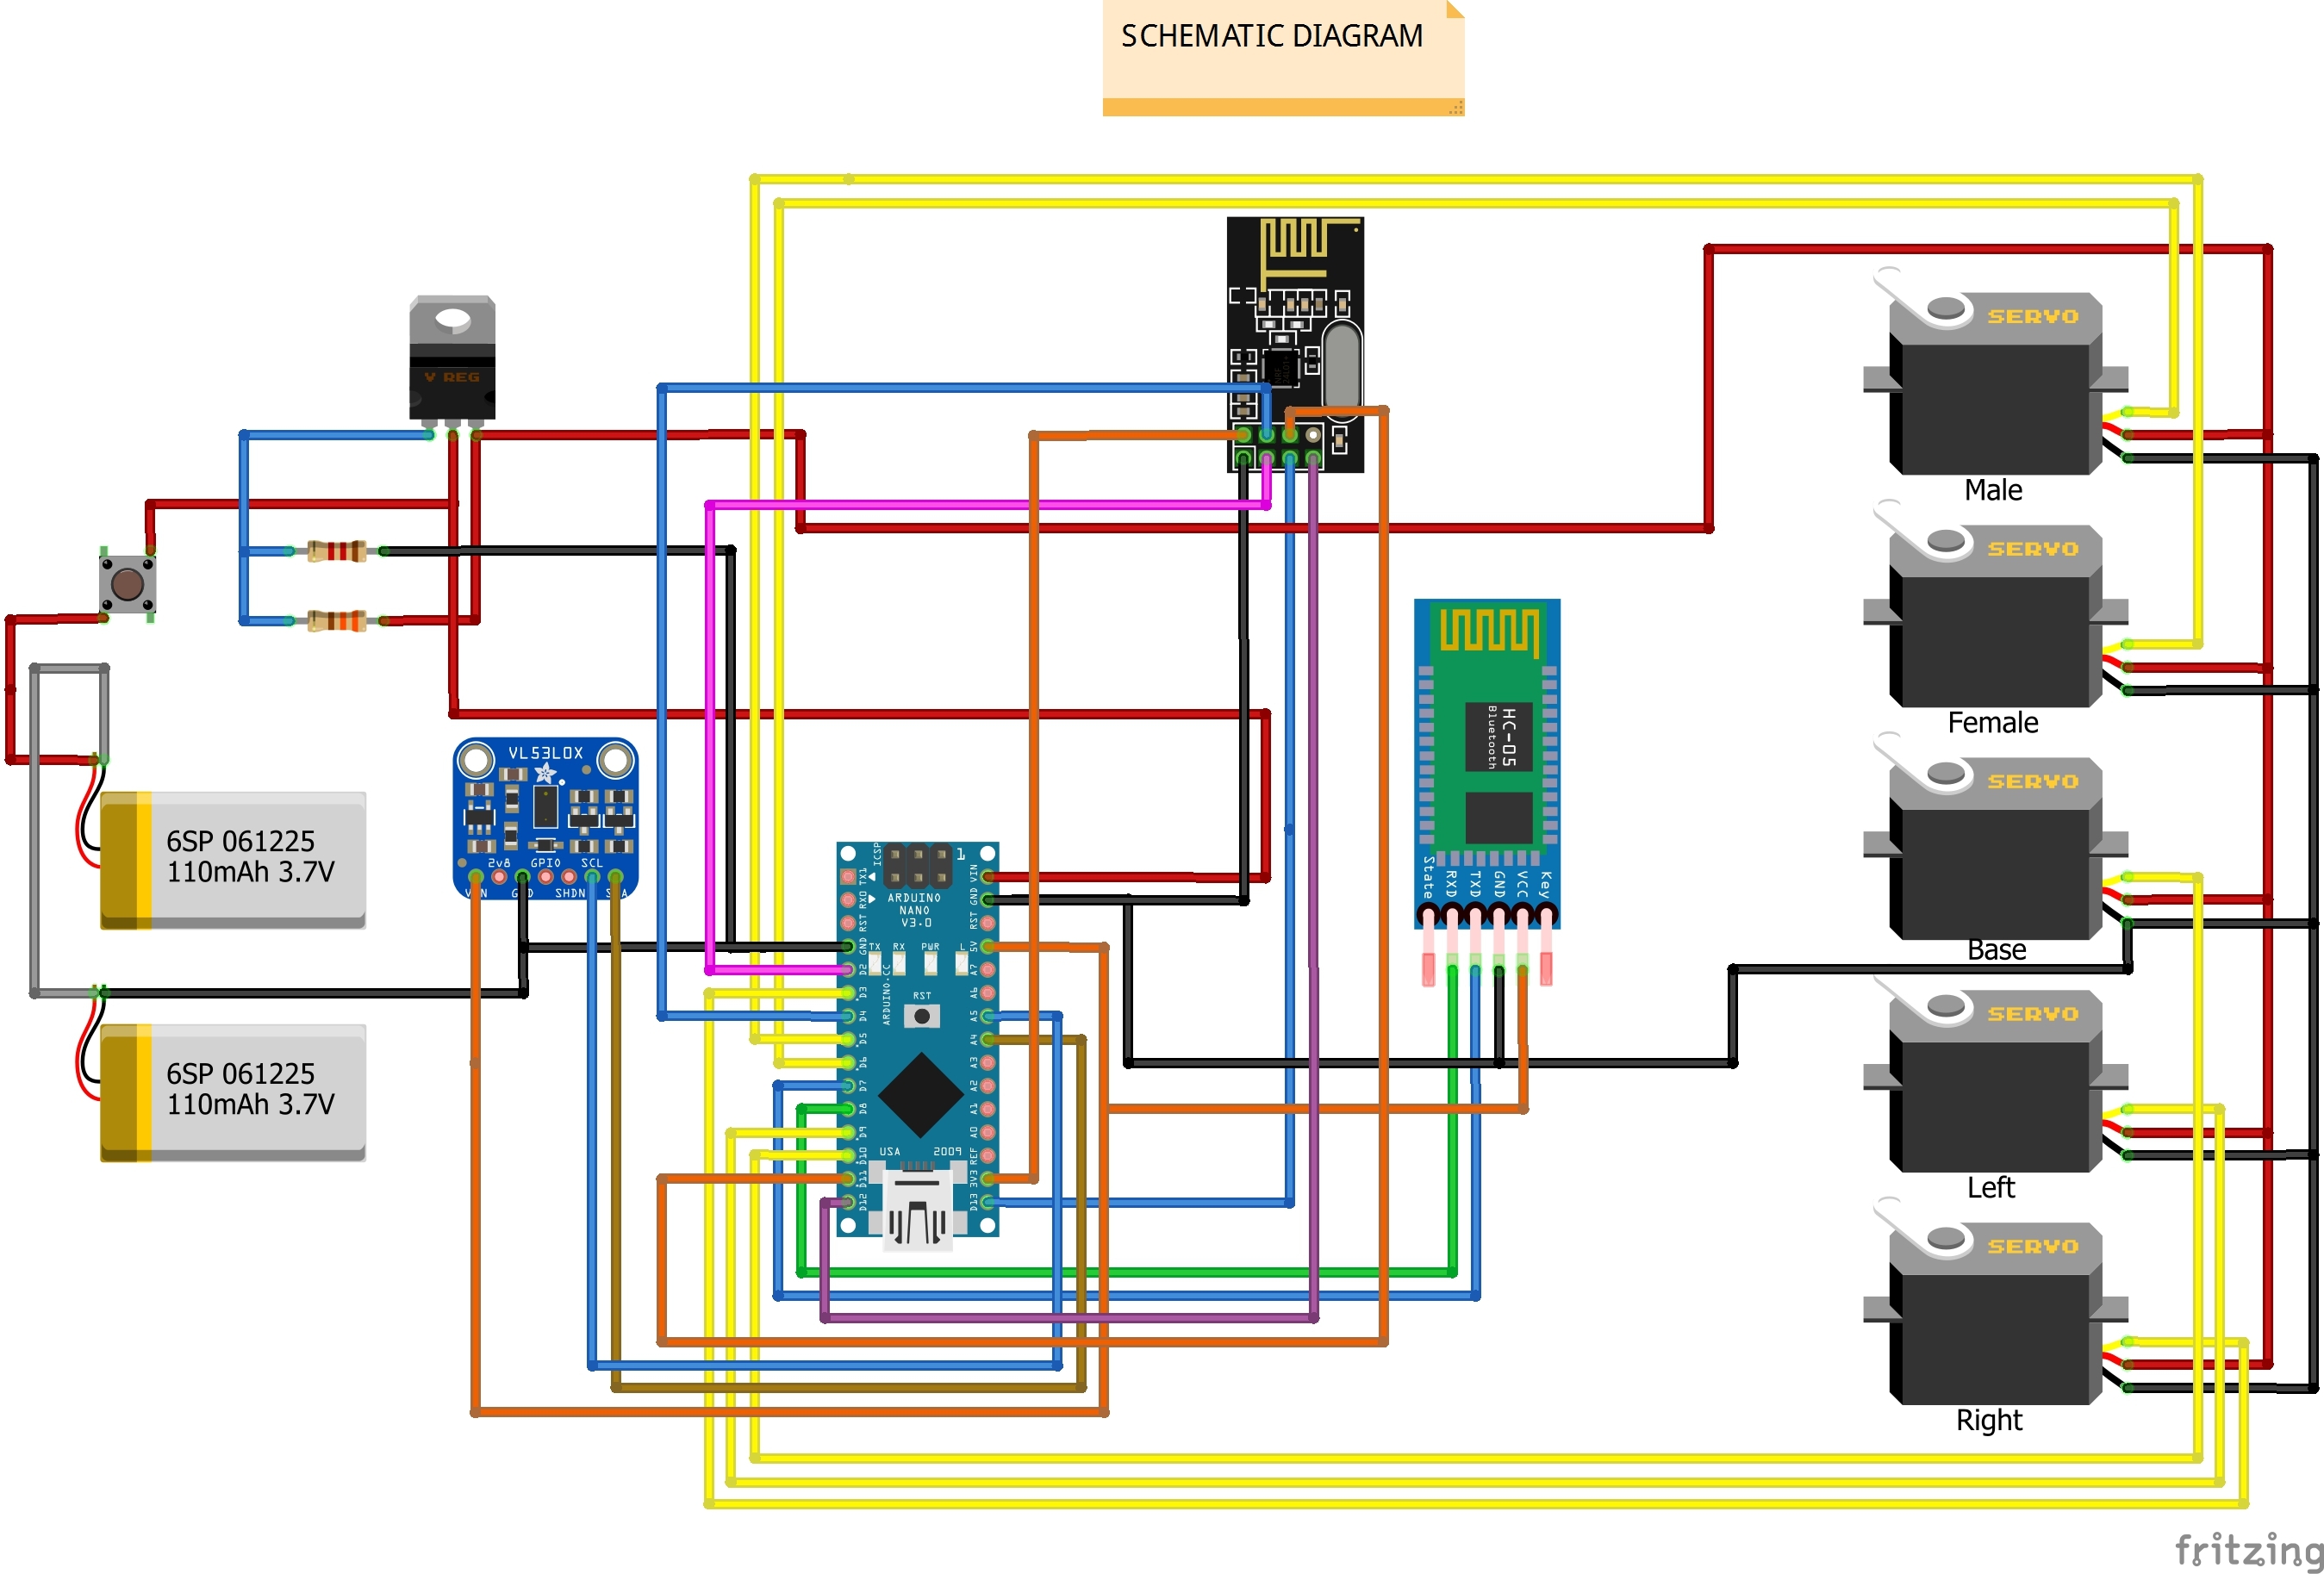
\includegraphics[scale=0.6]{Modular_Schematic_bb.jpg}

\subsection{Steps for assembly}
Steps for assembly can be found in this separate file \href{./Assembly steps for Dtto v2 Module.pdf}{here}.



\pagebreak

\section{Software and Code}

The program can be found in the eYSIP repository 
\href{https://github.com/eYSIP-2017/eYSIP-2017_Modular-Robot}{here}.\\

\noindent The entire program flow can be described by the flowcharts below:

\begin{itemize}

\item General flow \\
\begin{center}
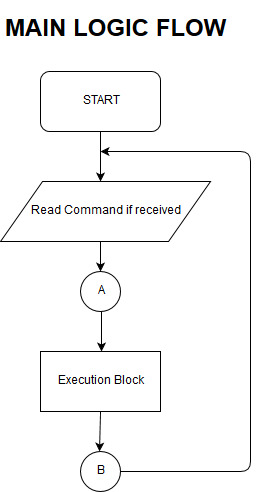
\includegraphics[scale=0.8]{main_flow2.jpg}
\end{center}
 

\end{itemize}
\pagebreak

\noindent The execution part can be elaborated further based on the type of command:

\begin{itemize}
\item Set angle \\

\vspace{-20pt}
\begin{center}
 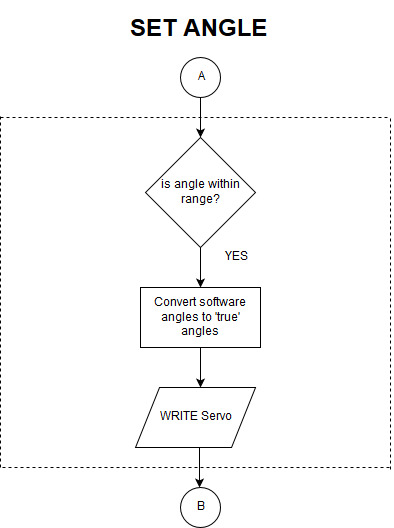
\includegraphics[scale=0.5]{set_angle_flow2.jpg}
\end{center}


\item Wheel \\
\vspace{-20pt}
\begin{center}
 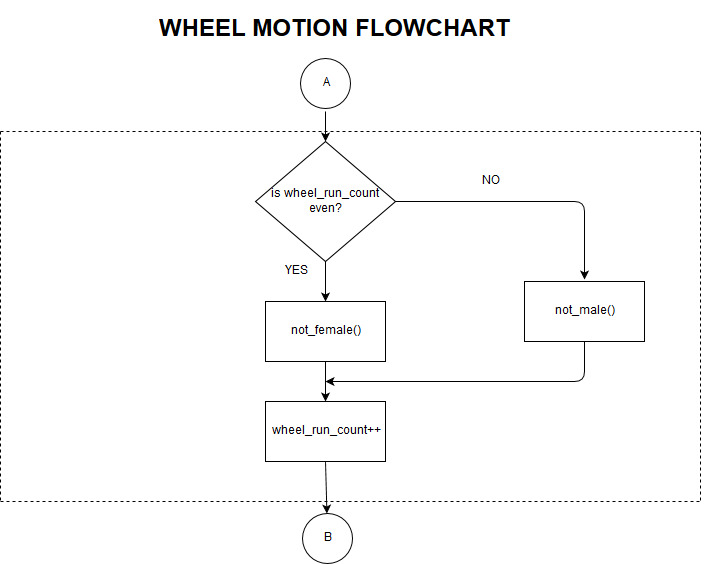
\includegraphics[scale=0.4]{wheel_flow2.jpg}
\end{center}



\item Snake \\
\begin{center}
 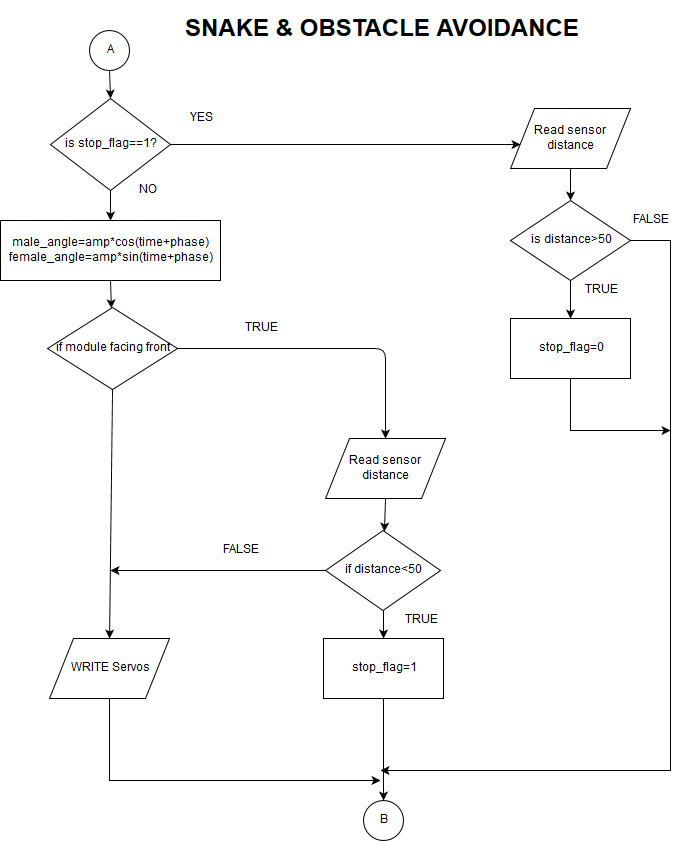
\includegraphics[scale=0.5]{snake_flow2.jpg}
\end{center}

\end{itemize}

\noindent Other than this, the entire code is well documented for detailed insights.

\pagebreak

\section{Use and Demo}
\subsection{Final Setup}
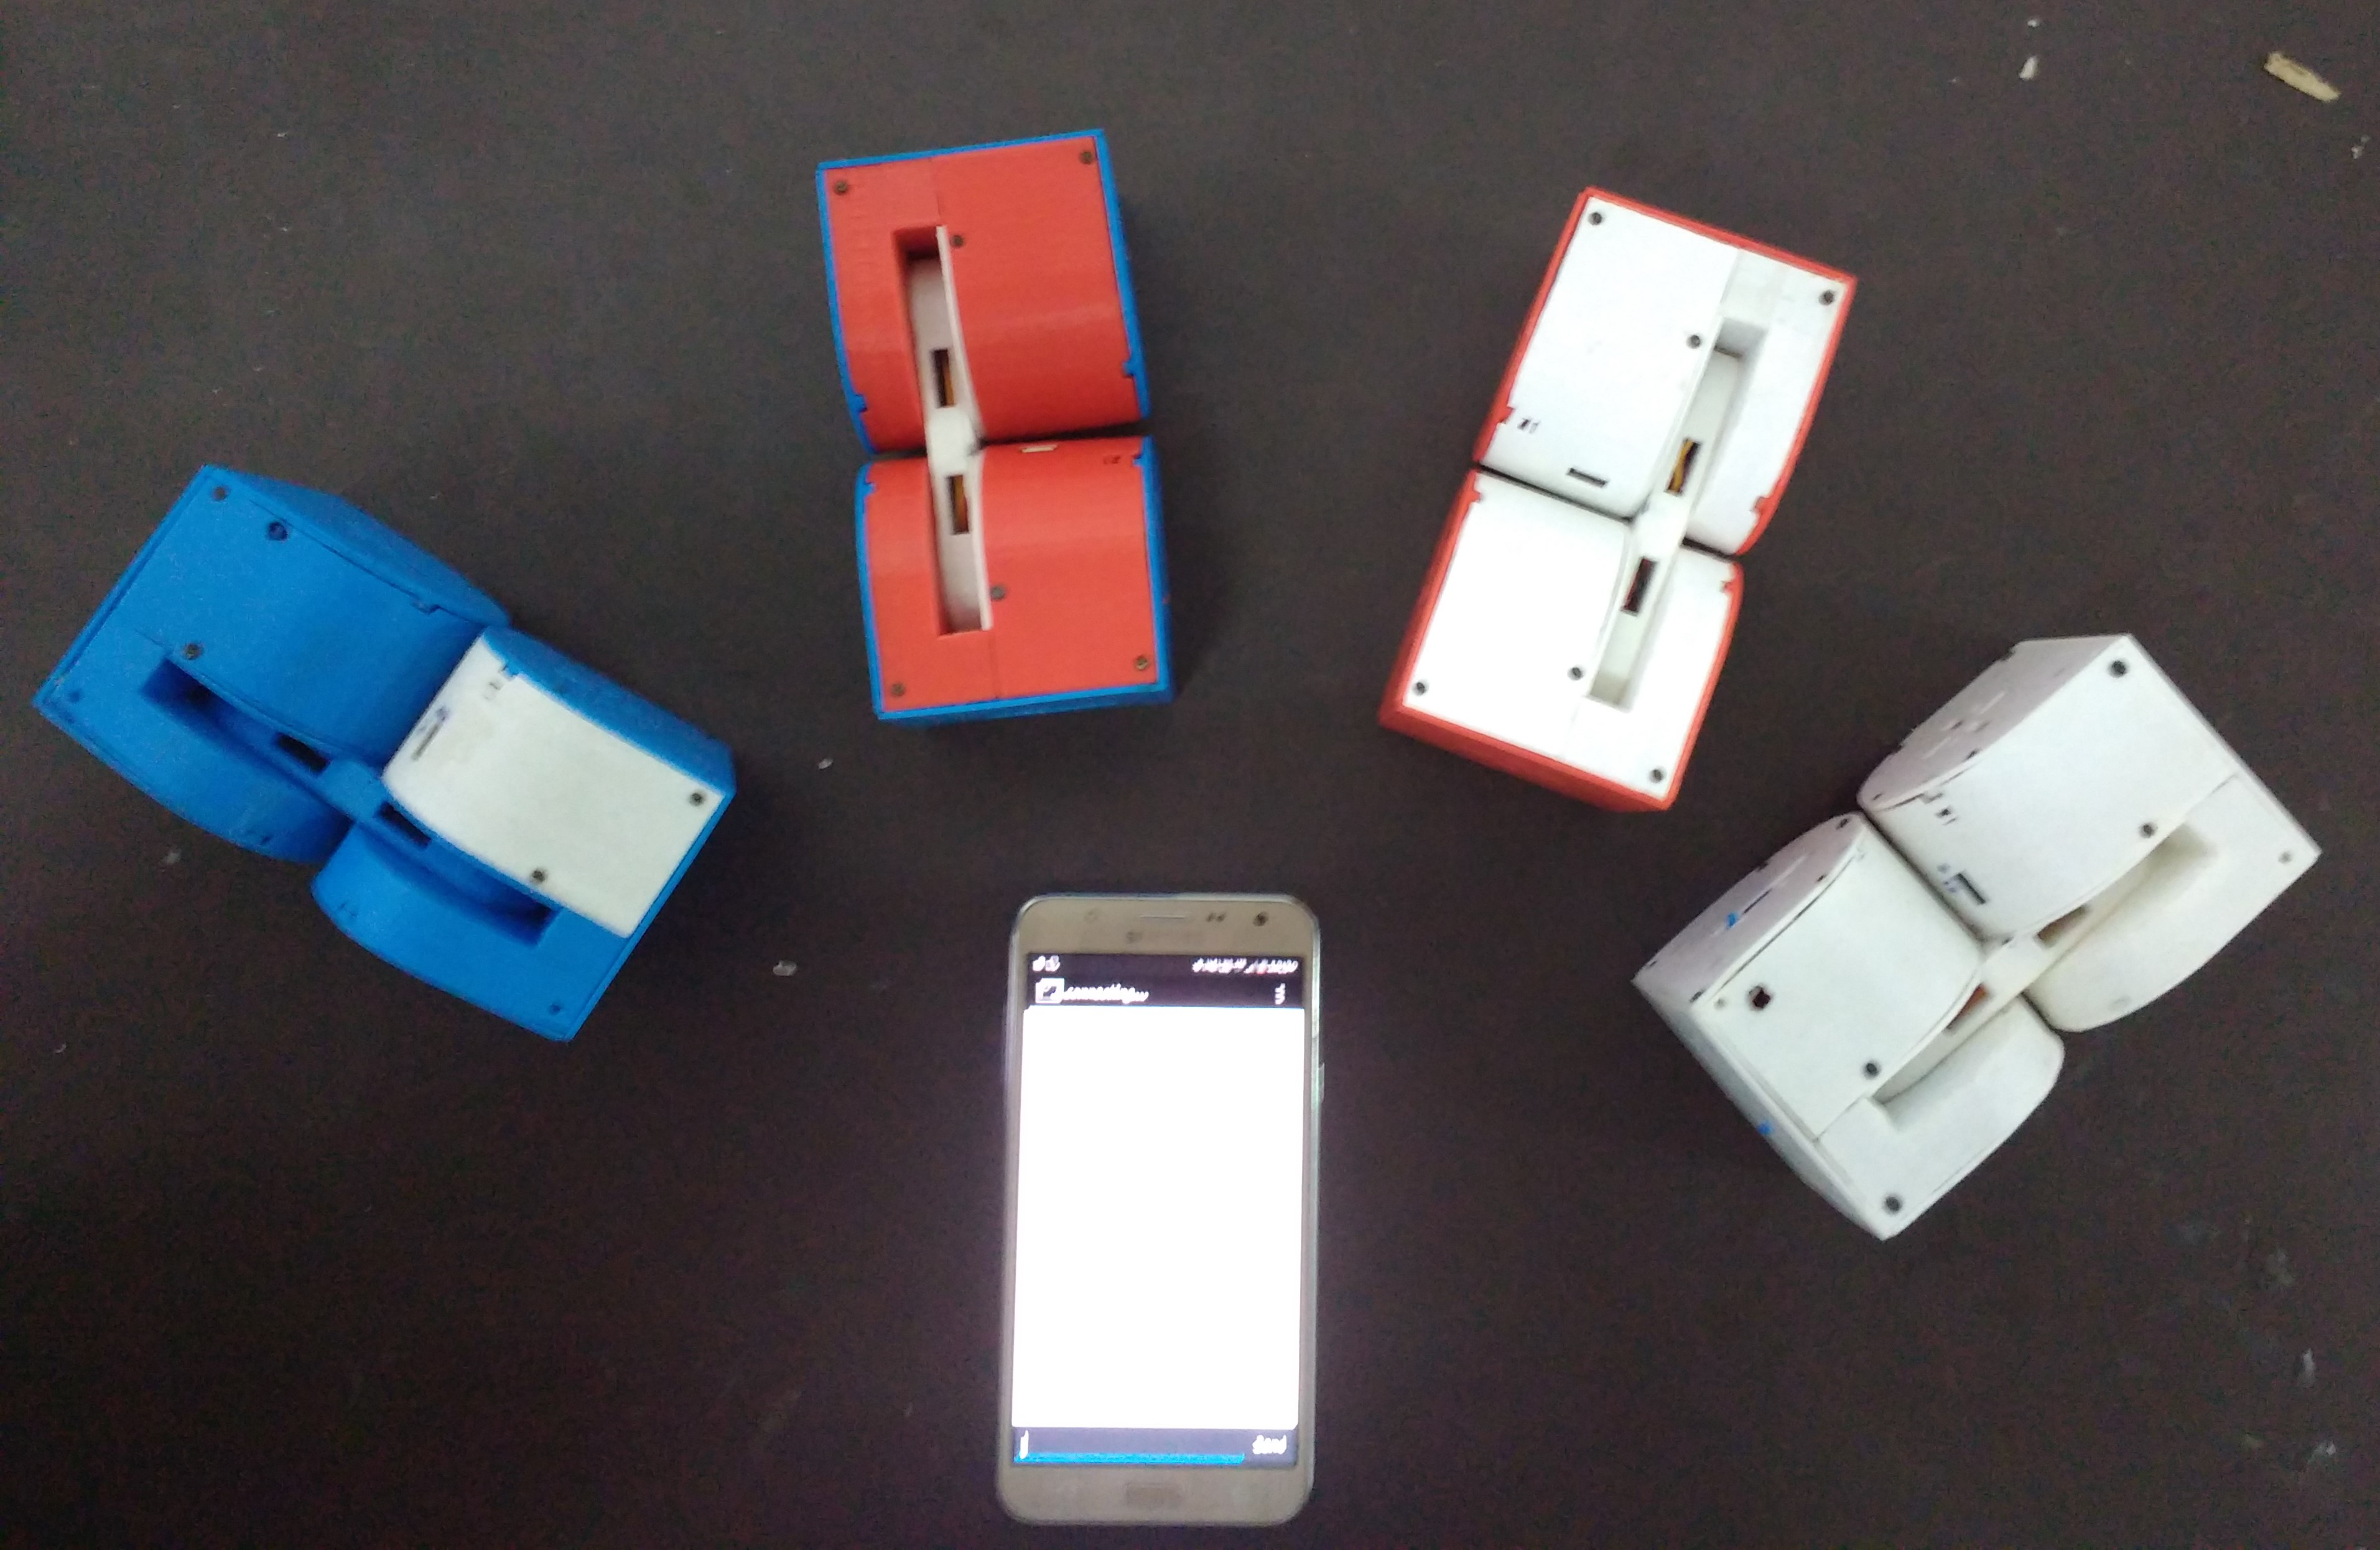
\includegraphics[scale=0.09]{final_setup.jpg}

\vspace{10pt}

\noindent The 4 Dtto modules assembled can be commanded using a Bluetooth device such as a smartphone shown above. The terminal application for Android devices can be downloaded \href{https://play.google.com/store/apps/details?id=Qwerty.BluetoothTerminal}{here}.

\subsection{User Instruction}
\noindent Load the Bluetooth Terminal application and connect to the master module from Options, Connect a device - Secure, 'Name of master HC-05'. Send the required commands. Best way to check all modules is by sending 'arm', which is to generate snake motion in all modules.

\vspace{10pt}

\noindent Structure of commands for controlling the Dtto using Bluetooth can be found in '\href{./Command_Definition.pdf}{Command\_Definitions.pdf}' present with this report or in our GitHub repository \href{https://github.com/eYSIP-2017/eYSIP-2017_Modular-Robot/blob/master/Final\%20Report/Command_Definition.pdf}{here}.

\subsection{Demonstration Video}
\begin{itemize}
\item \noindent Demonstration of snake motion and obstacle avoidance. \href{https://youtu.be/fWWrK-H1P5A}{\ExternalLink}

\item \noindent Demonstration of wheel motion. \href{https://youtu.be/WYdw9-lhOyw}{\ExternalLink}
\end{itemize}


\pagebreak

\section{Future Work}
There is vast amount of research and work which can be done
in the field of modular robotics and in our project, some 
enhancements which can be implemented in future are:

\begin{enumerate}
\item For faster processing and space saving, ESP8266/ESP32 can be used in place of Arduino Nano.

\item Using the basic modules implemented in the project with an overhead camera which can provide a reference frame for all modules.

\item Increasing the DOF of each module by adding rotating faces like the Dtto v3 which is under works.

\item Adding additional sensors for more feedback such as a  gravity sensor which can act as a reference for hinge angles.

\item Using a higher torque motor on the 'mega' modules being developed can add possibilities of different motions and transformations.
\end{enumerate}

\section{Bug report and Challenges}
\begin{itemize}
\item Appropriate screws (M1.7 x 4mm Flathead) were unavailable, so the CAD design was modified multiple times and the printing and assembly of modules was delayed.

\item The specified servo motor, MG92B is unavailable in local and online stores in India, so we're forced to use a lower torque motor MG90S, which is the closest that can be fit under the given module dimensions. Because of this many of the transformations was not possible.
\end{itemize}

\begin{thebibliography}{li}

\bibitem{dtto_alberto}
Alberto,
{\em Dtto - Explorer Modular Robot},
2016. \href{https://hackaday.io/project/9976-dtto-explorer-modular-robot}{\ExternalLink}

\bibitem{vrep_manual} 
V-REP User Manual. \href{http://www.coppeliarobotics.com/helpFiles/}{\ExternalLink}

\bibitem{hc05}
HC-05 specifications and AT commands. \href{https://www.itead.cc/wiki/Serial_Port_Bluetooth_Module_(Master/Slave)_:_HC-05}{\ExternalLink}

\bibitem{servo_cad}
Servo SG90, 3D CAD model. \href{https://grabcad.com/library/tower-pro-sg92r-servo-motor-1}{\ExternalLink}



\end{thebibliography}


\end{document}

